\renewcommand{\baselinestretch}{2} \small\normalsize
\chapter{Propagation Statistics}
This chapter describes the propagation factor statistics after numerically propagating over independent random sea surface realizations in a Monte Carlo fashion.

\section{Sampling Constraints}
The initial set of runs was performed at Ka-Band (35 GHz). The mean and standard deviation for a 100 run Monte Carlo set are shown in Figure \ref{stat_fig:1}. This data set took over 48 hours to complete running on a laptop and the results were washed out at near range (Figure \ref{stat_fig:1} is clipped at 10 km downrange).

\begin{figure}[H]
  \begin{center}
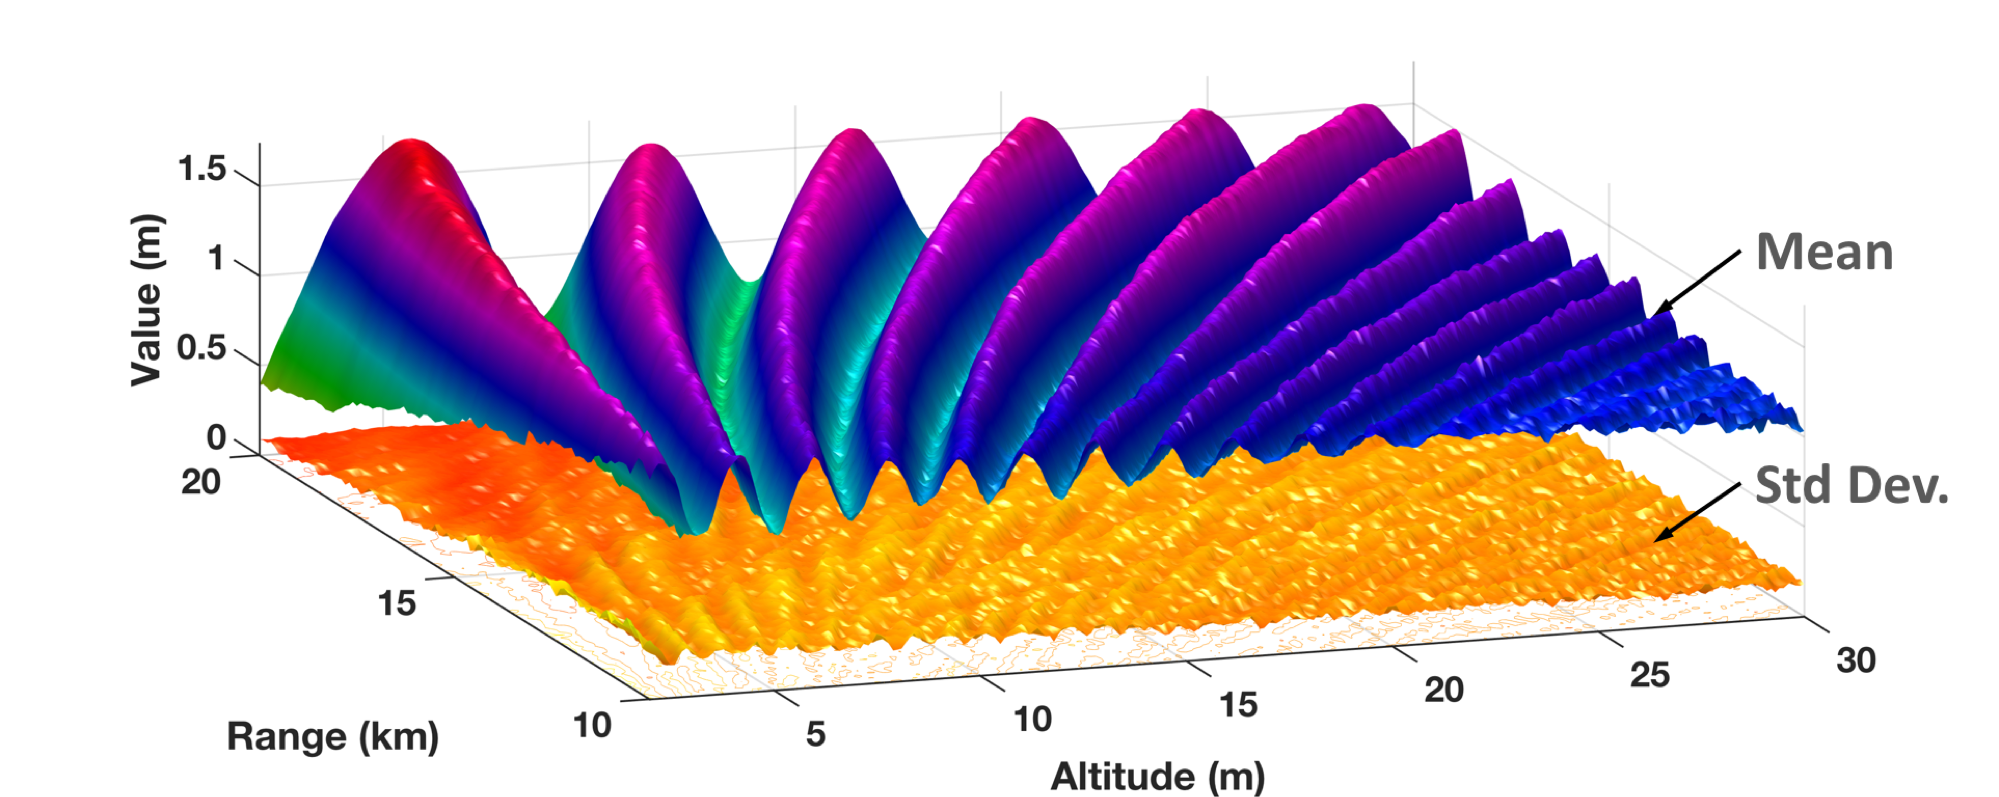
\includegraphics[width=5in]{../media/statistics/ka_band_stats.png}
  \end{center}
  \renewcommand{\baselinestretch}{1} \small\normalsize
  \begin{quote}
    \caption[Ensemble Statistics at Ka-Band]{Ensemble Statistics at Ka-Band\label{stat_fig:1}}
  \end{quote}
\end{figure}
\renewcommand{\baselinestretch}{2} \small\normalsize

Figure \ref{stat_fig:2} shows the mean and standard deviation for a 100 run Monte Carlo set at X-band (10 GHz). In this case, the near range results are much cleaner and the data set took less than 6 hours to complete.
\begin{figure}[H]
  \begin{center}
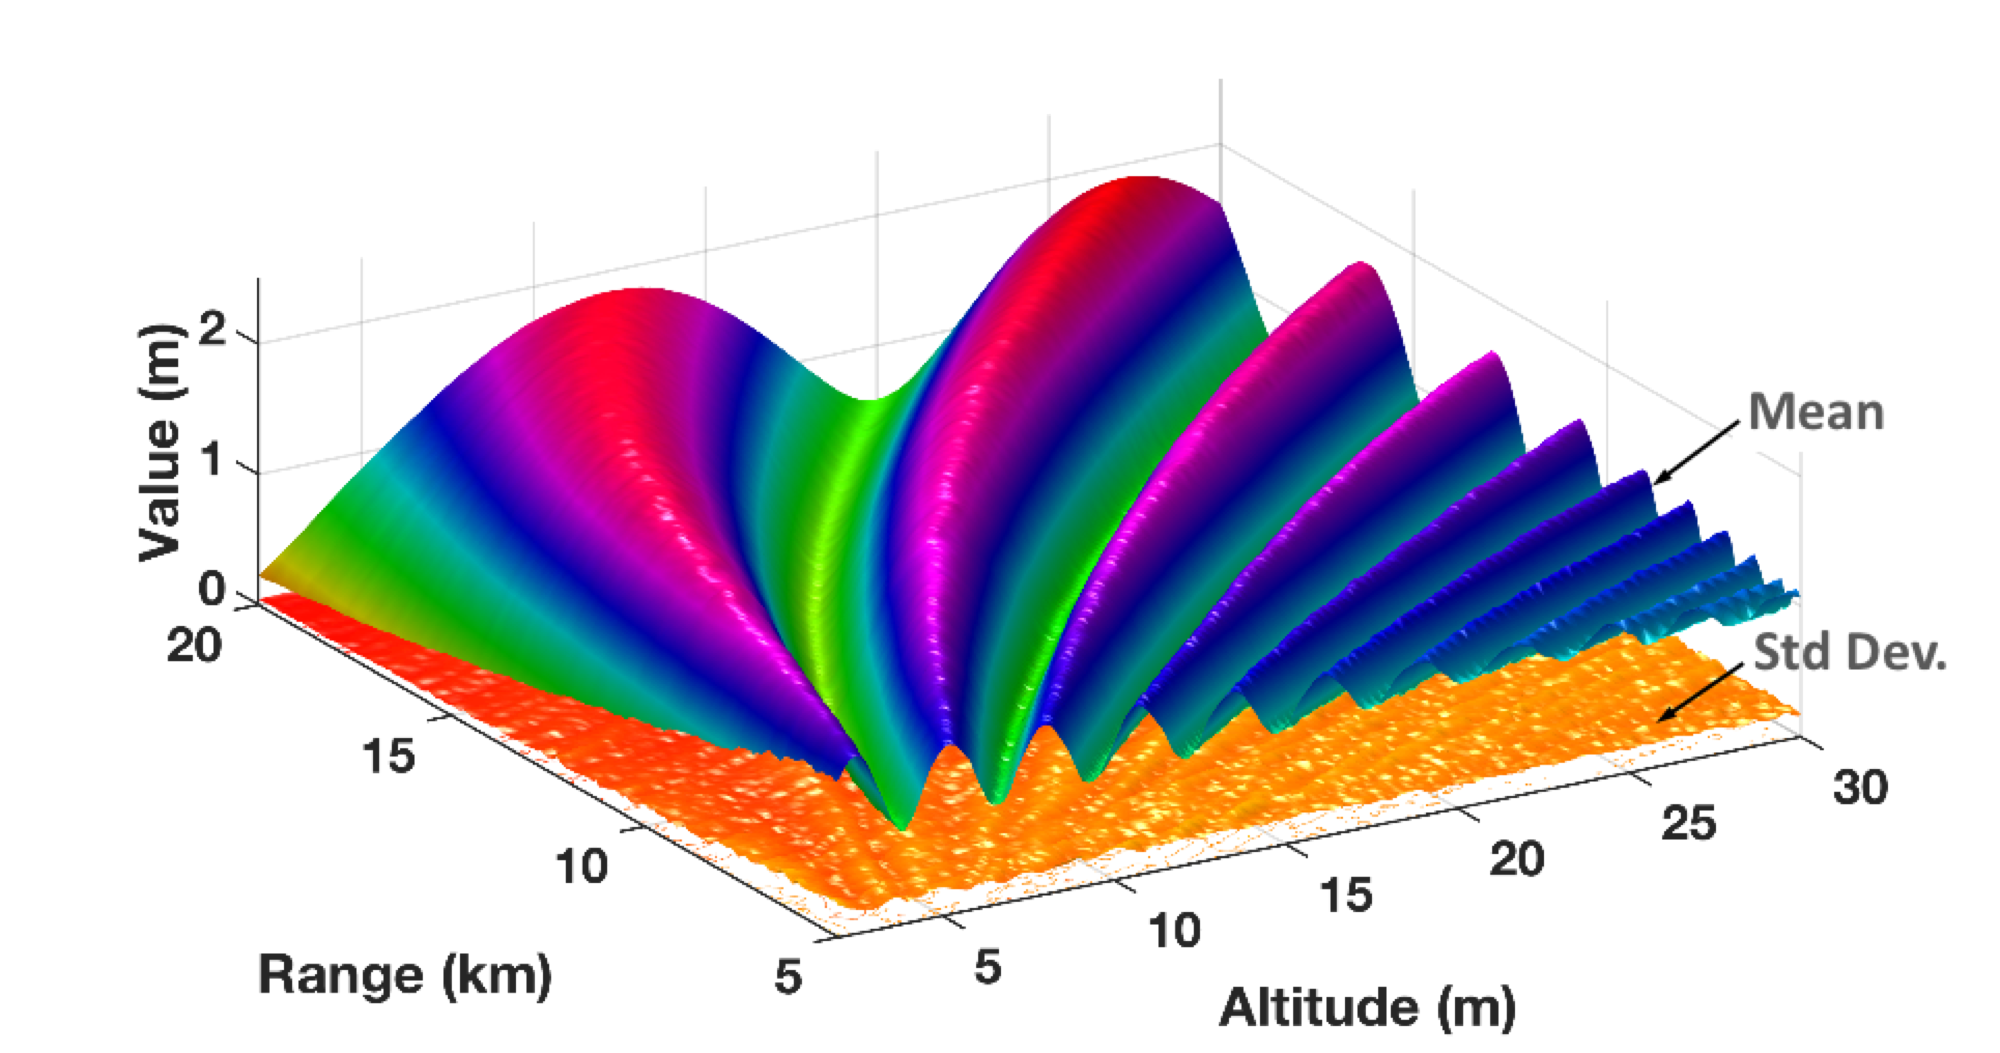
\includegraphics[width=5in]{../media/statistics/x_band_stats.png}
  \end{center}
  \renewcommand{\baselinestretch}{1} \small\normalsize
  \begin{quote}
    \caption[Ensemble Statistics at X-Band]{Ensemble Statistics at X-Band\label{stat_fig:2}}
  \end{quote}
\end{figure}
\renewcommand{\baselinestretch}{2} \small\normalsize

These results indicate that spatial sampling constraints from numerical propagation are important for obtaining accurate statistics, so we need to understand those impacts. From the propagation factor for the 2 ray model, $F_p = e^{jkL_1} + \Gamma_1e^{jkL_{so}}$, we can look at the phase difference between the two primary paths, $\Delta\varphi = k\left[ L_1 - L_{so}\right]$.
\begin{equation}
\boxed{\Delta\varphi = -\frac{4\pi h_1h_2}{\lambda L}}
\label{stat_eq:1}
\end{equation}
\renewcommand{\baselinestretch}{2} \small\normalsize

\noindent The derivative of the phase difference with respect to range is then
\begin{equation}
\frac{d\Delta\varphi}{dL}=-\frac{4\pi h_1h_2}{\lambda L^2}
\label{stat_eq:2}
\end{equation}
\renewcommand{\baselinestretch}{2} \small\normalsize

\noindent This can be converted from rad/m to rad/sample by multiplying by the spatial sampling distance in range, $\Delta L$. We can insist that this phase shift per sample be smaller than some pre-determined value to provide adequate sampling. It is often convenient to specify a limit in terms of wavelengths and we can enforce the condition that there must be at least $n$ samples per wavelength by letting

\begin{equation}
\frac{4\pi h_1h_2\Delta L}{\lambda L^2} \leq \frac{2\pi \lambda}{n}
\label{stat_eq:3}
\end{equation}

This yields a constraint for the maximum allowable spatial sampling step to ensure $n$ samples per wavelength.
\begin{equation}
\boxed{\Delta L \leq \frac{\lambda^2 L^2}{2nh_1h_2}}
\label{stat_eq:4}
\end{equation}

This sampling constraint is shown in Figure \ref{stat_fig:3} for both the 10 and 35 GHz cases, with $n = 20$ and $\delta r = 0.5$.

\begin{figure}[H]
  \begin{center}
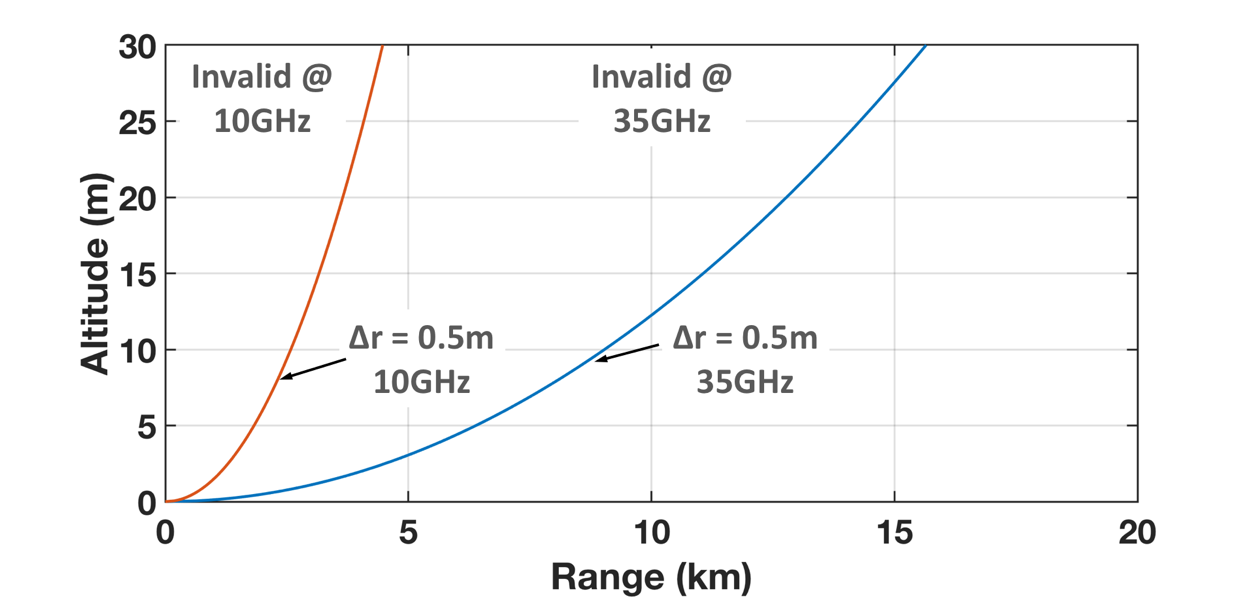
\includegraphics[width=5in]{../media/statistics/sampling_constraint.png}
  \end{center}
  \renewcommand{\baselinestretch}{1} \small\normalsize
  \begin{quote}
    \caption[Sampling Constraints for Statistical Analysis]{Sampling Constraints for Statistical Analysis\label{stat_fig:3}}
  \end{quote}
\end{figure}
\renewcommand{\baselinestretch}{2} \small\normalsize

Figure \ref{stat_fig:1a} and Figure \ref{stat_fig:1b} show example propagation factors from two specific sea surface realizations.

\section{Monte Carlo Run Results}
\begin{figure}[H]
  \begin{center}
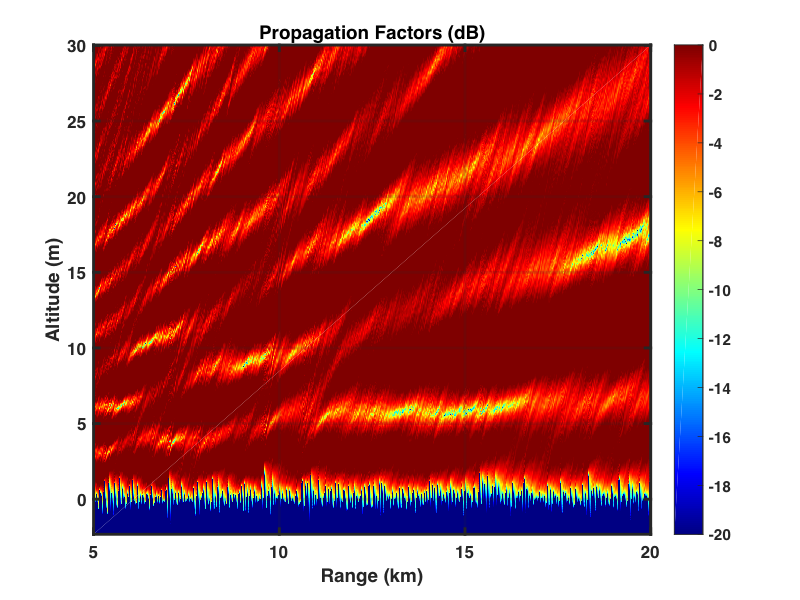
\includegraphics[width=5in]{../media/statistics/pf_1.png}
  \end{center}
  \renewcommand{\baselinestretch}{1} \small\normalsize
  \begin{quote}
    \caption[Example Propagation Factor Realization]{Example Propagation Factor Realization\label{stat_fig:1a}}
  \end{quote}
\end{figure}
\renewcommand{\baselinestretch}{2} \small\normalsize

\begin{figure}[H]
  \begin{center}
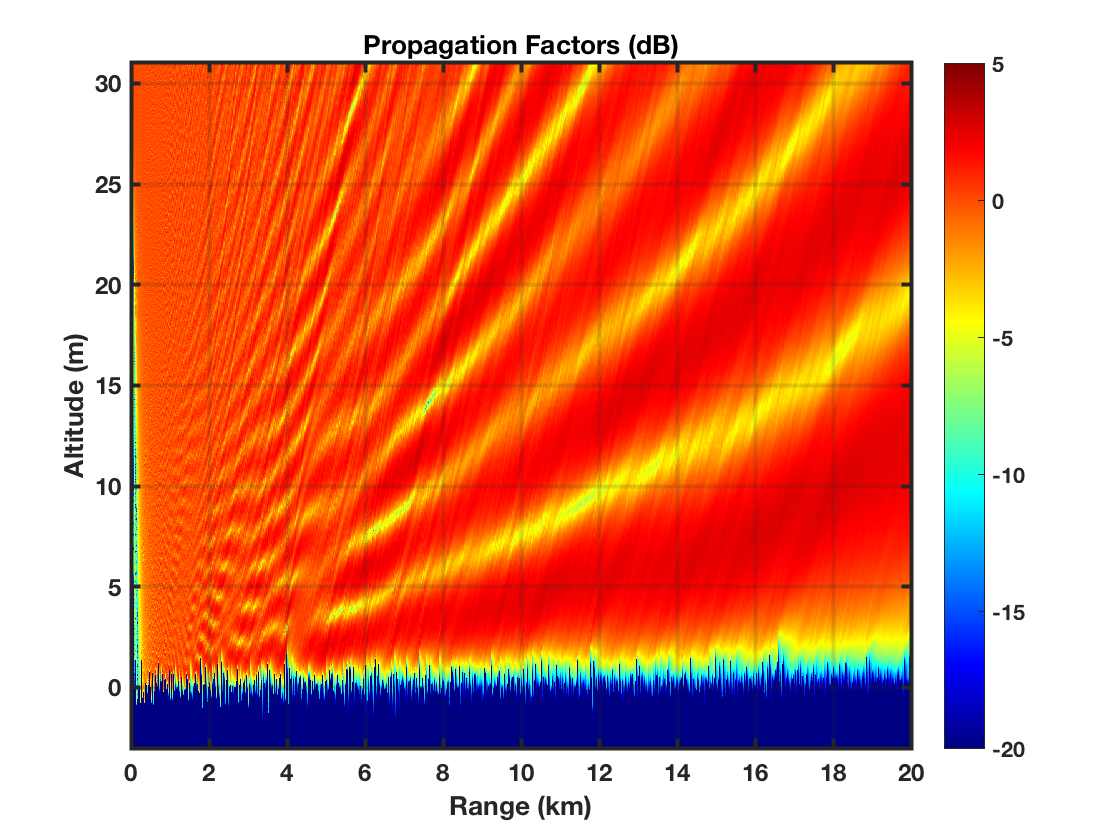
\includegraphics[width=5in]{../media/statistics/pf_2.png}
  \end{center}
  \renewcommand{\baselinestretch}{1} \small\normalsize
  \begin{quote}
    \caption[Example Propagation Factor Realization]{Example Propagation Factor Realization\label{stat_fig:1b}}
  \end{quote}
\end{figure}
\renewcommand{\baselinestretch}{2} \small\normalsize

\section{PDF Fitting Results}
As shown in \cite{yeh_first_principles} and \cite{yeh_fading}, we expect the statistics to follow a Rician distribution

\begin{equation}
P = \frac{x}{\sigma^2}\exp\left[\frac{-(x^2 + \nu^2}{2\sigma^2} \right]I_0\left(\frac{x\nu}{\sigma} \right)
\label{stat_eq:3}
\end{equation}
\renewcommand{\baselinestretch}{2} \small\normalsize

\begin{figure}[H]
  \begin{center}
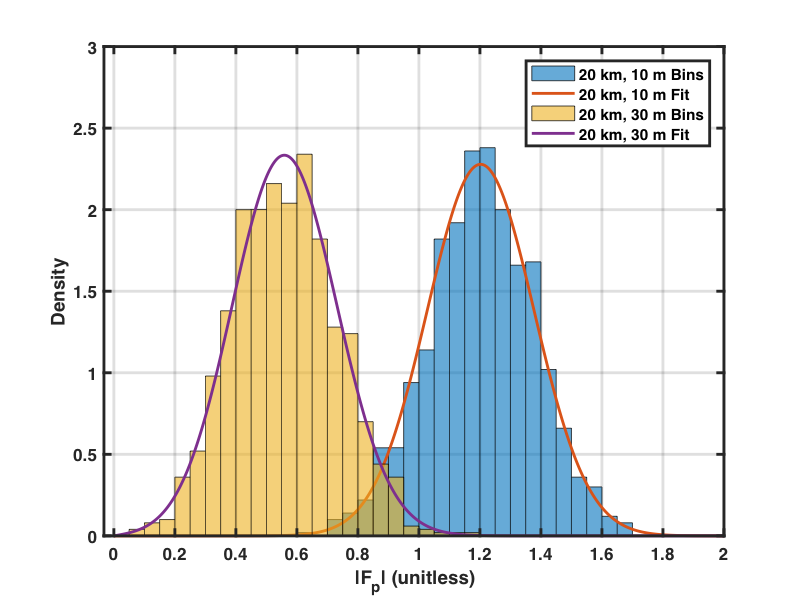
\includegraphics[width=5in]{../media/statistics/constant_range_fit.png}
  \end{center}
  \renewcommand{\baselinestretch}{1} \small\normalsize
  \begin{quote}
    \caption[PDF Fitting at Constant Range]{PDF Fitting at Constant Range\label{stat_fig:4}}
  \end{quote}
\end{figure}
\renewcommand{\baselinestretch}{2} \small\normalsize

\begin{figure}[H]
  \begin{center}
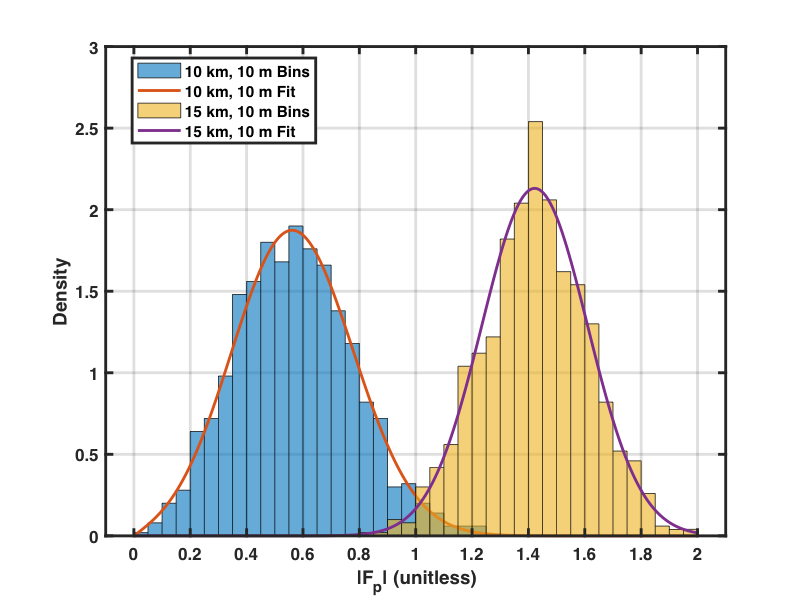
\includegraphics[width=5in]{../media/statistics/constant_altitude_fit.png}
  \end{center}
  \renewcommand{\baselinestretch}{1} \small\normalsize
  \begin{quote}
    \caption[PDF Fitting at Constant Altitude]{PDF Fitting at Constant Altitude\label{stat_fig:5}}
  \end{quote}
\end{figure}
\renewcommand{\baselinestretch}{2} \small\normalsize
